\documentclass{beamer}
% Some basic packages
\usepackage[utf8]{inputenc}
\usepackage[T1]{fontenc}
\usepackage{textcomp}
\usepackage[english]{babel}
\usepackage{url}
\usepackage{graphicx}
\usepackage{float}
\usepackage{booktabs}
\usepackage{enumitem}

%\pdfminorversion=7

% for algorithm typing
\usepackage[vlined]{algorithm2e}
\SetKw{KwBy}{by}

% Don't indent paragraphs, leave some space between them
%\usepackage{parskip}

% Hide page number when page is empty
%\usepackage{emptypage}
\usepackage{subcaption}
\usepackage{multicol}
\usepackage{xcolor}

% Other font I sometimes use.
% \usepackage{cmbright}
\usefonttheme[onlymath]{serif}

% Math stuff
\usepackage{amsmath, amsfonts, mathtools, amsthm, amssymb}
% Fancy script capitals
\usepackage{mathrsfs}
\usepackage{cancel}
% Bold math
\usepackage{bm}
% Some shortcuts
\newcommand\N{\ensuremath{\mathbb{N}}}
\newcommand\R{\ensuremath{\mathbb{R}}}
\newcommand\Z{\ensuremath{\mathbb{Z}}}
\renewcommand\O{\ensuremath{\emptyset}}
\newcommand\Q{\ensuremath{\mathbb{Q}}}
\newcommand\C{\ensuremath{\mathbb{C}}}
\renewcommand\L{\ensuremath{\mathcal{L}}}

% Easily typeset systems of equations (French package)
\usepackage{systeme}

% Put x \to \infty below \lim
\let\svlim\lim\def\lim{\svlim\limits}

%Make implies and impliedby shorter
\let\implies\Rightarrow
\let\impliedby\Leftarrow
\let\iff\Leftrightarrow
\let\epsilon\varepsilon

% Add \contra symbol to denote contradiction
\usepackage{stmaryrd} % for \lightning
\newcommand\contra{\scalebox{1.5}{$\lightning$}}

% \let\phi\varphi

% Command for short corrections
% Usage: 1+1=\correct{3}{2}

\definecolor{correct}{HTML}{009900}
\newcommand\correct[2]{\ensuremath{\:}{\color{red}{#1}}\ensuremath{\to }{\color{correct}{#2}}\ensuremath{\:}}
\newcommand\green[1]{{\color{correct}{#1}}}

% horizontal rule
\newcommand\hr{
    \noindent\rule[0.5ex]{\linewidth}{0.5pt}
}

% hide parts
\newcommand\hide[1]{}

% si unitx
\usepackage{siunitx}
\sisetup{locale = FR}

% Environments
%\makeatother
% For box around Definition, Theorem, \ldots
%\usepackage{mdframed}
%\mdfsetup{skipabove=1em,skipbelow=0em}
%\theoremstyle{definition}

%\newmdtheoremenv[nobreak=true]{definition}{Definition}
%\newmdtheoremenv[nobreak=true]{note}{Note}
%\newtheorem*{eg}{Example}
%\newtheorem*{notation}{Notation}
%\newtheorem*{previouslyseen}{As previously seen}
%\newtheorem*{remark}{Remark}
%\newtheorem*{problem}{Problem}
%\newtheorem*{observe}{Observe}
%\newtheorem*{property}{Property}
%\newtheorem*{intuition}{Intuition}
%\newmdtheoremenv[nobreak=true]{prop}{Proposition}
%\newmdtheoremenv[nobreak=true]{theorem}{Theorem}
%\newmdtheoremenv[nobreak=true]{corollary}{Corollary}

% End example and intermezzo environments with a small diamond (just like proof
% environments end with a small square)
%\usepackage{etoolbox}
%\AtEndEnvironment{vb}{\null\hfill$\diamond$}%
%\AtEndEnvironment{intermezzo}{\null\hfill$\diamond$}%
% \AtEndEnvironment{opmerking}{\null\hfill$\diamond$}%

% Fix some spacing
% http://tex.stackexchange.com/questions/22119/how-can-i-change-the-spacing-before-theorems-with-amsthm
%\makeatletter
%\def\thm@space@setup{%
%  \thm@preskip=\parskip \thm@postskip=0pt
%}


% Exercise 
% Usage:
% \exercise{5}
% \subexercise{1}
% \subexercise{2}
% \subexercise{3}
% gives
% Exercise 5
%   Exercise 5.1
%   Exercise 5.2
%   Exercise 5.3
%\newcommand{\exercise}[1]{%
%    \def\@exercise{#1}%
%    \subsection*{Exercise #1}
%}
%
%\newcommand{\subexercise}[1]{%
%    \subsubsection*{Exercise \@exercise.#1}
%}


% \lecture starts a new lecture (les in dutch)
%
% Usage:
% \lecture{1}{di 12 feb 2019 16:00}{Inleiding}
%
% This adds a section heading with the number / title of the lecture and a
% margin paragraph with the date.

% I use \dateparts here to hide the year (2019). This way, I can easily parse
% the date of each lecture unambiguously while still having a human-friendly
% short format printed to the pdf.

%\usepackage{xifthen}
%\def\testdateparts#1{\dateparts#1\relax}
%\def\dateparts#1 #2 #3 #4 #5\relax{
%    \marginpar{\small\textsf{\mbox{#1 #2 #3 #5}}}
%}

%\def\@lecture{}%
%\newcommand{\lecture}[3]{
%    \ifthenelse{\isempty{#3}}{%
%        \def\@lecture{Lecture #1}%
%    }{%
%        \def\@lecture{Lecture #1: #3}%
%    }%
%    \section{\@lecture}
%    \marginpar{\small\textsf{\mbox{#2}}}
%}



% These are the fancy headers
%\usepackage{fancyhdr}
%\pagestyle{fancy}

% LE: left even
% RO: right odd
% CE, CO: center even, center odd
% My name for when I print my lecture notes to use for an open book exam.
% \fancyhead[LE,RO]{Gilles Castel}

%\fancyhead[RO,LE]{\@lecture} % Right odd,  Left even
%\fancyhead[RE,LO]{}          % Right even, Left odd
%
%\fancyfoot[RO,LE]{\thepage}  % Right odd,  Left even
%\fancyfoot[RE,LO]{}          % Right even, Left odd
%\fancyfoot[C]{\leftmark}     % Center
%
%\makeatother




% Todonotes and inline notes in fancy boxes
\usepackage{todonotes}
\usepackage{tcolorbox}

% Make boxes breakable
\tcbuselibrary{breakable}

% Verbetering is correction in Dutch
% Usage: 
% \begin{verbetering}
%     Lorem ipsum dolor sit amet, consetetur sadipscing elitr, sed diam nonumy eirmod
%     tempor invidunt ut labore et dolore magna aliquyam erat, sed diam voluptua. At
%     vero eos et accusam et justo duo dolores et ea rebum. Stet clita kasd gubergren,
%     no sea takimata sanctus est Lorem ipsum dolor sit amet.
% \end{verbetering}
%\newenvironment{verbetering}{\begin{tcolorbox}[
%    arc=0mm,
%    colback=white,
%    colframe=green!60!black,
%    title=Opmerking,
%    fonttitle=\sffamily,
%    breakable
%]}{\end{tcolorbox}}

% Noot is note in Dutch. Same as 'verbetering' but color of box is different
%\newenvironment{noot}[1]{\begin{tcolorbox}[
%    arc=0mm,
%    colback=white,
%    colframe=white!60!black,
%    title=#1,
%    fonttitle=\sffamily,
%    breakable
%]}{\end{tcolorbox}}




% Figure support as explained in my blog post.
%\usepackage{import}
%\usepackage{xifthen}
%\usepackage{pdfpages}
%\usepackage{transparent}
%\newcommand{\incfig}[1]{%
%    \def\svgwidth{\columnwidth}
%    \import{./figures/}{#1.pdf_tex}
%}

% Fix some stuff
% %http://tex.stackexchange.com/questions/76273/multiple-pdfs-with-page-group-included-in-a-single-page-warning
\pdfsuppresswarningpagegroup=1


% My name
\author{Bruno M. Pacheco}

% Fixes sections starting at 0
%\setcounter{chapter}{1}% Not using chapters, but they're used in the counters

% Hides the numbers of sections but keeps them at the toc
%\setcounter{secnumdepth}{0}

% Add ToC to beginning of each section
\AtBeginSection[]{
    \begin{frame}
	\frametitle{Agenda}
	\tableofcontents[currentsection]
    \end{frame}
}

\graphicspath{{./figures/}}

\title[FFT]{Fast Fourier Transform Algorithm}
\date{2021.1}

\RestyleAlgo{ruled}

\begin{document}

% make title frame
\frame{\titlepage}

% make ToC
\begin{frame}
    \frametitle{Agenda}
    \tableofcontents
\end{frame}

\section{Fourier Transform}

\subsection{(Continuous) Fourier Transform}

\begin{frame}
    \frametitle{Disclaimer}
    \begin{alertblock}{Be Aware!}
	We will handle frequency in radians per second for the entire presentation, so lots of $2\pi$ will show up. It is for the greater good.
    \end{alertblock}
\end{frame}

\begin{frame}
    \frametitle{A review on Fourier transform and analysis}
    An integrable function $x: T \longrightarrow \R$ over a continuous interval $T$ can be expressed as a Fourier series \[
    x(t) = a_0 + \sum_{n=1}^{\infty} a_n \cos n\omega_0 t + b_n \sin n\omega_0 t
    ,\] where $\omega_0 = \frac{2\pi}{|T|}$ is the frequency step and
    \begin{align*}
        a_n &= \frac{2}{|T|} \int_T x(t) \cos n\omega_0 t \,dt \\
        b_n &= \frac{2}{|T|} \int_T x(t) \sin n\omega_0 t \,dt
    .\end{align*}
\end{frame}

\begin{frame}
    \frametitle{A review on Fourier transform and analysis}
    \begin{figure}
        \centering
        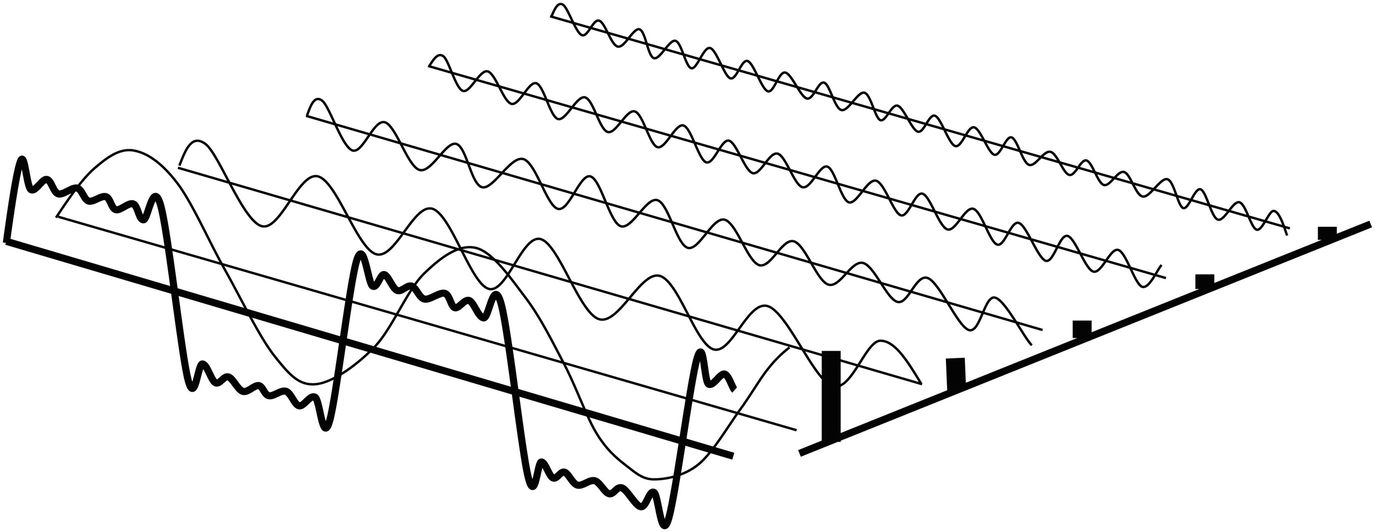
\includegraphics[width=0.8\textwidth]{fourier_series.png}
        \caption{First 5 terms of the Fourier series expansion of a square wave.}
        \label{fig:fourier_series-png}
    \end{figure}
\end{frame}

\begin{frame}
    \frametitle{Exponential form of the Fourier series}
    If we apply Euler's identity ($e^{i \pi} = \cos x + i \sin x$), we get \[
    x(t) = \sum_{n=1}^{\infty} c_n e^{i \omega_0 n t}
    ,\] where \[
    c_n = \frac{1}{|T|} \int_T x(t) e^{-i\omega_0 n t} \,dt
    .\] Note that, \[
	T\to \infty \implies \omega_0 \to 0
    ,\] that is, the series expansion of the whole signal will use all frequencies, which gets us to the intuition behind the Fourier transform.
\end{frame}

\begin{frame}
    \begin{exampleblock}{Fourier Transform}
     \[
    x(t) \xrightarrow{\mathcal{F}} X\left( \omega \right) = \int_{-\infty}^{\infty} x(t) e^{-i\omega t} \,dt
    \]
    \end{exampleblock}
     Note that $X\left( \omega \right) \in \C$, where $\Re\left\{ X\left( \omega \right)  \right\} $ is the magnitude and $\Im\left\{ X\left( \omega \right)  \right\} $ is the phase.
    Also, the inverse transform is very similar: \[
    X(\omega) \xrightarrow{\mathcal{F}^{-1}} x\left( t \right) = \frac{1}{2\pi}\int_{-\infty}^{\infty} X\left( \omega \right)  e^{i\omega t} \,d\omega
    .\] 
\end{frame}

\begin{frame}
    \frametitle{Fourier transform properties}
    There are several properties and they are quite similar to those of the Laplace transform. Given two integrable functions $x_1,x_2$ and $a,b \in \R$,
    \begin{description}
        \item[Linearity] \[
		a x_1(t) + bx_2(t) \xleftrightarrow{\mathcal{F}} aX_1\left( \omega \right) + bX_2\left( \omega \right) 
       \] 
       \item[Convolution] \[
	       x_1(t) * x_2(t)\xleftrightarrow{\mathcal{F}} X_1\left( \omega \right) X_2\left( \omega \right) 
       \] 
    \end{description}
\end{frame}

\subsection{Discrete Fourier Transform}

\begin{frame}
    \frametitle{Discrete Fourier Transform (DFT)}
    In computational machines, one needs the Fourier transform between discrete \emph{signals} and \emph{spectra}.
\end{frame}

\begin{frame}
    \frametitle{Discrete Fourier Transform (DFT)}
    Given an integrable function $x: \R \longrightarrow \R$ (signal), the N-sampled signal will be \[
	    \overline{x}(t) = \sum_{n=0}^{N-1} x\left( n T_s \right) \delta \left( t - n T_s \right) 
	,\] where $T_s \in \R$ is the sampling period and $N\in \N$ is the number of samples.

    \begin{figure}
	\centering
	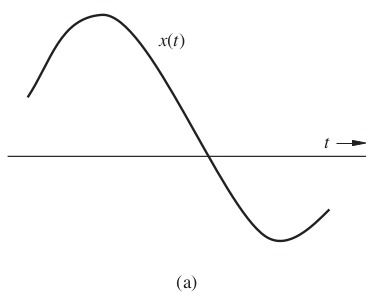
\includegraphics[width=0.35\textwidth]{fft_sampling_signal_a.png}
	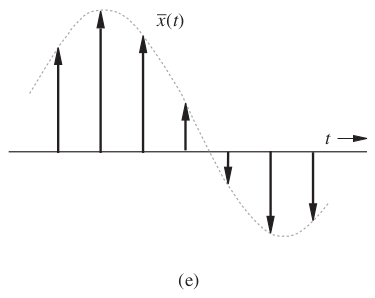
\includegraphics[width=0.35\textwidth]{fft_sampling_signal_b.png}
	\caption{Sampled signal example.}
	\label{fig:fft_sampling_signal_b-png}
    \end{figure}
\end{frame}

\begin{frame}
    \frametitle{Discrete Fourier Transform (DFT)}
    Now,\[
	\overline{x}(t) \xrightarrow{\mathcal{F}} \overline{X}\left( \omega \right) =\sum_{n=0}^{N-1} x\left( n T_s \right) e^{-i\omega n T_s}
    .\]
    At the same time, we know that, assuming a high enough sampling frequency, by Nyquist, $X\left( \omega \right) = T_s \overline{X}\left( \omega \right)$, thus, \[
    X\left( \omega \right) = T_s \sum_{n=0}^{N-1} x\left( n T_s \right) e^{-i\omega n T_s}
    .\] 
\end{frame}

\begin{frame}
    \frametitle{Discrete Fourier Transform (DFT)}
    Note that, for a sampling frequency of $\frac{1}{T_s}$ and $N$ samples, by Nyquist, the minimum frequency that can be characterized is \[
    \omega_s = \frac{2\pi}{N T_s}
    \] and is defined by the length of the signal (just like in the Fourier series).
\end{frame}

\begin{frame}
    \frametitle{Discrete Fourier Transform (DFT)}
    Also by Nyquist, we know that for any finite sampling frequency, one can have multiple fitting harmonics, so the frequency spectrum will repeat itself every $\frac{2\pi}{T_s}$ interval.
    \begin{figure}[H]
        \centering
        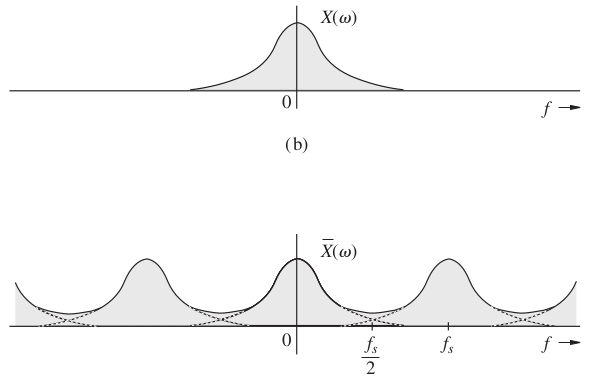
\includegraphics[width=0.6\textwidth]{frequency_spectrum_repeating.png}
        \caption{Frequency spectrum of a sampled signal.}
        \label{fig:frequency_spectrum_repeating-pn}
    \end{figure}
\end{frame}

\begin{frame}
    \frametitle{Discrete Fourier Transform (DFT)}
    Therefore, we are interested in as many $\omega_s$ samples fit in the $\frac{2\pi}{T_s}$ frequency interval, which happens to be \[
    \frac{\frac{2\pi}{T_s}}{\omega_s} =\frac{\frac{2\pi}{T_s}}{\frac{2\pi}{N T_s}} = N
    ,\] that is, there are as many samples in the frequency spectrum as in the sampled signal.
\end{frame}

\begin{frame}
    \frametitle{DFT Notation}
    Finally, to make things easier, we  will define $x_n = T_s x\left( n T_s \right)$ and $X_r = X\left( r \omega_s \right) $, which will give us the final definition for the DFT:
    \begin{exampleblock}{DFT}
        Given a signal $x$ with $N$ samples every $T_s$ seconds, \[
        X_r = \sum_{n=0}^{N-1} x_{n} W_N^{r n}
        ,\] where \[
	    W_N = e^{-i\omega_s T_s} = e^{-\frac{2\pi i}{N}}
        .\] 
    \end{exampleblock}
\end{frame}

\begin{frame}
    \frametitle{DFT Notation}
    \begin{exampleblock}{DFT}
        Given a signal $x$ with $N$ samples every $T_s$ seconds, \[
        X_r = \sum_{n=0}^{N-1} x_{n} W_N^{r n}
        .\]
    \end{exampleblock}
    \begin{figure}
        \centering
        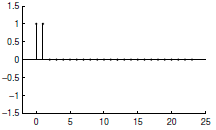
\includegraphics[width=0.4\textwidth]{dft_a.png}
        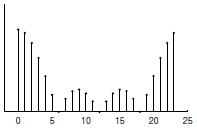
\includegraphics[width=0.4\textwidth]{dft_b.png}
        \caption{Example of a sampled signal and its discrete frequency spectrum.}
        \label{fig:dft_b-png}
    \end{figure}
\end{frame}

\begin{frame}
    \frametitle{DFT Complexity}
    \begin{exampleblock}{DFT}
        \[
        X_r = \sum_{n=0}^{N-1} x_{n} W_N^{r n}
        \]
    \end{exampleblock}
    For the above definition, each frequency will require $N-1$ summations, and $2N$ multiplications. As one must compute $N$ frequency values, the DFT has \textbf{$\Theta\left( n^2 \right) $ complexity}.
\end{frame}

\section{Fast Fourier Transform}

\subsection{Linearity of the DFT}

\begin{frame}
    \frametitle{Linearity of the DFT}
    It is trivial to see that the DFT, as the Fourier Transform, is a linear operator, that is, \[
	a x_{n}^1 + bx_{m}^2 \xleftrightarrow{\mathcal{F}} aX_r^1 + bX_q^2
    .\] 
\end{frame}

\begin{frame}
    \frametitle{Linearity of the DFT}
    From this, we will see that it is possible to compute the DFT of a signal from two DFT of two smaller signals.

    Let us assume $N$ is a power of two and split $x_{n}$ into $x_{2m}$ and $x_{2m+1}$. From this,
    \begin{align*}
        X_r &= \sum_{n=0}^{N-1} x_{n} W_N^{r n} \\
	&= \sum_{m=0}^{\frac{N}{2}-1} x_{2m} W_N^{r 2m} + \sum_{m=0}^{\frac{N}{2}-1} x_{2m+1}W_N^{r\left( 2m+1 \right) } \\
	&= \sum_{m=0}^{\frac{N}{2}-1} x_{2m} W_N^{r 2m} + W_N^{r}			\sum_{m=0}^{\frac{N}{2}-1} x_{2m+1}W_N^{r2m}
    .\end{align*}
\end{frame}

\begin{frame}
    \frametitle{Linearity of the DFT}
    But \[
    W_N^{r 2m} = e^{-\frac{2\pi i}{N} r 2m} = e^{-\frac{2\pi i}{\frac{N}{2}} r m} = W_{\frac{N}{2}}^{rm}
    ,\] thus
    \begin{align*}
	X_r &= \sum_{m=0}^{\frac{N}{2}-1} x_{2m} W_N^{r 2m} + W_N^{r}			\sum_{m=0}^{\frac{N}{2}-1} x_{2m+1}W_N^{r2m} \\
	    &= \underbrace{\sum_{m=0}^{\frac{N}{2}-1} x_{2m} W_{\frac{N}{2}}^{r m}}_{\text{DFT of }x_{2m}} + W_N^{r}\underbrace{\sum_{m=0}^{\frac{N}{2}-1} x_{2m+1}W_{\frac{N}{2}}^{rm}}_{\text{DFT of }x_{2m+1}}
    .\end{align*}
\end{frame}

\begin{frame}
    \frametitle{Linearity of the DFT}
    Even more, as the complex exponential is periodical (remember $e^{\pi i} = -1$), we can see that
    \begin{align*}
        X_{r+\frac{N}{2}} &= \sum_{m=0}^{\frac{N}{2}-1} x_{2m} W_N^{\left( r + \frac{N}{2} \right)  2m} + \sum_{m=0}^{\frac{N}{2}-1} x_{2m+1}W_N^{\left( r + \frac{N}{2} \right)\left( 2m+1 \right) } \\
	&= \sum_{m=0}^{\frac{N}{2}-1} x_{2m} W_N^{r 2m} W_N^{N m} + W_N^{r+\frac{N}{2}}\sum_{m=0}^{\frac{N}{2}-1} x_{2m+1}W_N^{r2m}W_N^{N m}
    .\end{align*}
\end{frame}

\begin{frame}
    \frametitle{Linearity of the DFT}
    Still, \[
	W_N^{N m} = e^{-\frac{2\pi i}{N} N m} = e^{-2 \pi i m} = 1
    \] and \[
	W_N^{\frac{N}{2}} = e^{-\pi i} = -1 \implies W_N^{r + \frac{N}{2}} = -W_N^{r}
    .\] Therefore, \[
	X_{r+\frac{N}{2}}= \underbrace{\sum_{m=0}^{\frac{N}{2}-1} x_{2m} W_{\frac{N}{2}}^{r m}}_{\text{DFT of }x_{2m}} - W_N^{r}\underbrace{\sum_{m=0}^{\frac{N}{2}-1} x_{2m+1}W_{\frac{N}{2}}^{rm}}_{\text{DFT of }x_{2m+1}}
    .\] 
\end{frame}

\subsection{The Cooley-Tukey algorithm}
\begin{frame}
    \frametitle{The Cooley-Tukey algorithm}
    These properties form a butterfly relation between the inputs and outputs of the DFT for a pair of frequencies.
    \begin{figure}
        \centering
        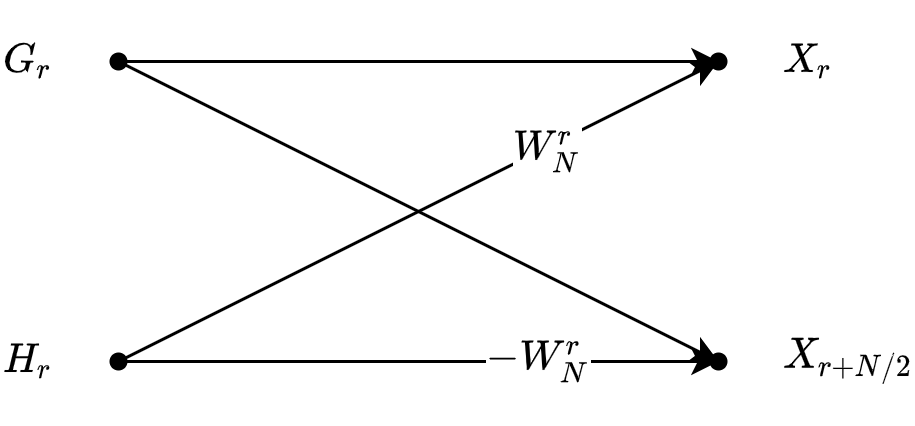
\includegraphics[width=0.8\textwidth]{cooleytukey_butterfly.png}
	\caption{Relation between $G_r$ and $H_r$ the DFTs of $x_{2m}$ and $x_{2m+1}$ resp. and two values of $X_r$.}
        \label{fig:cooleytukey_butterfly-png}
    \end{figure}
\end{frame}

\begin{frame}
    \frametitle{The Cooley-Tukey algorithm}
    Even further, one can apply the same properties to both $G_r$ and $H_r$, up to $\log N$ times.
    \begin{figure}
        \centering
        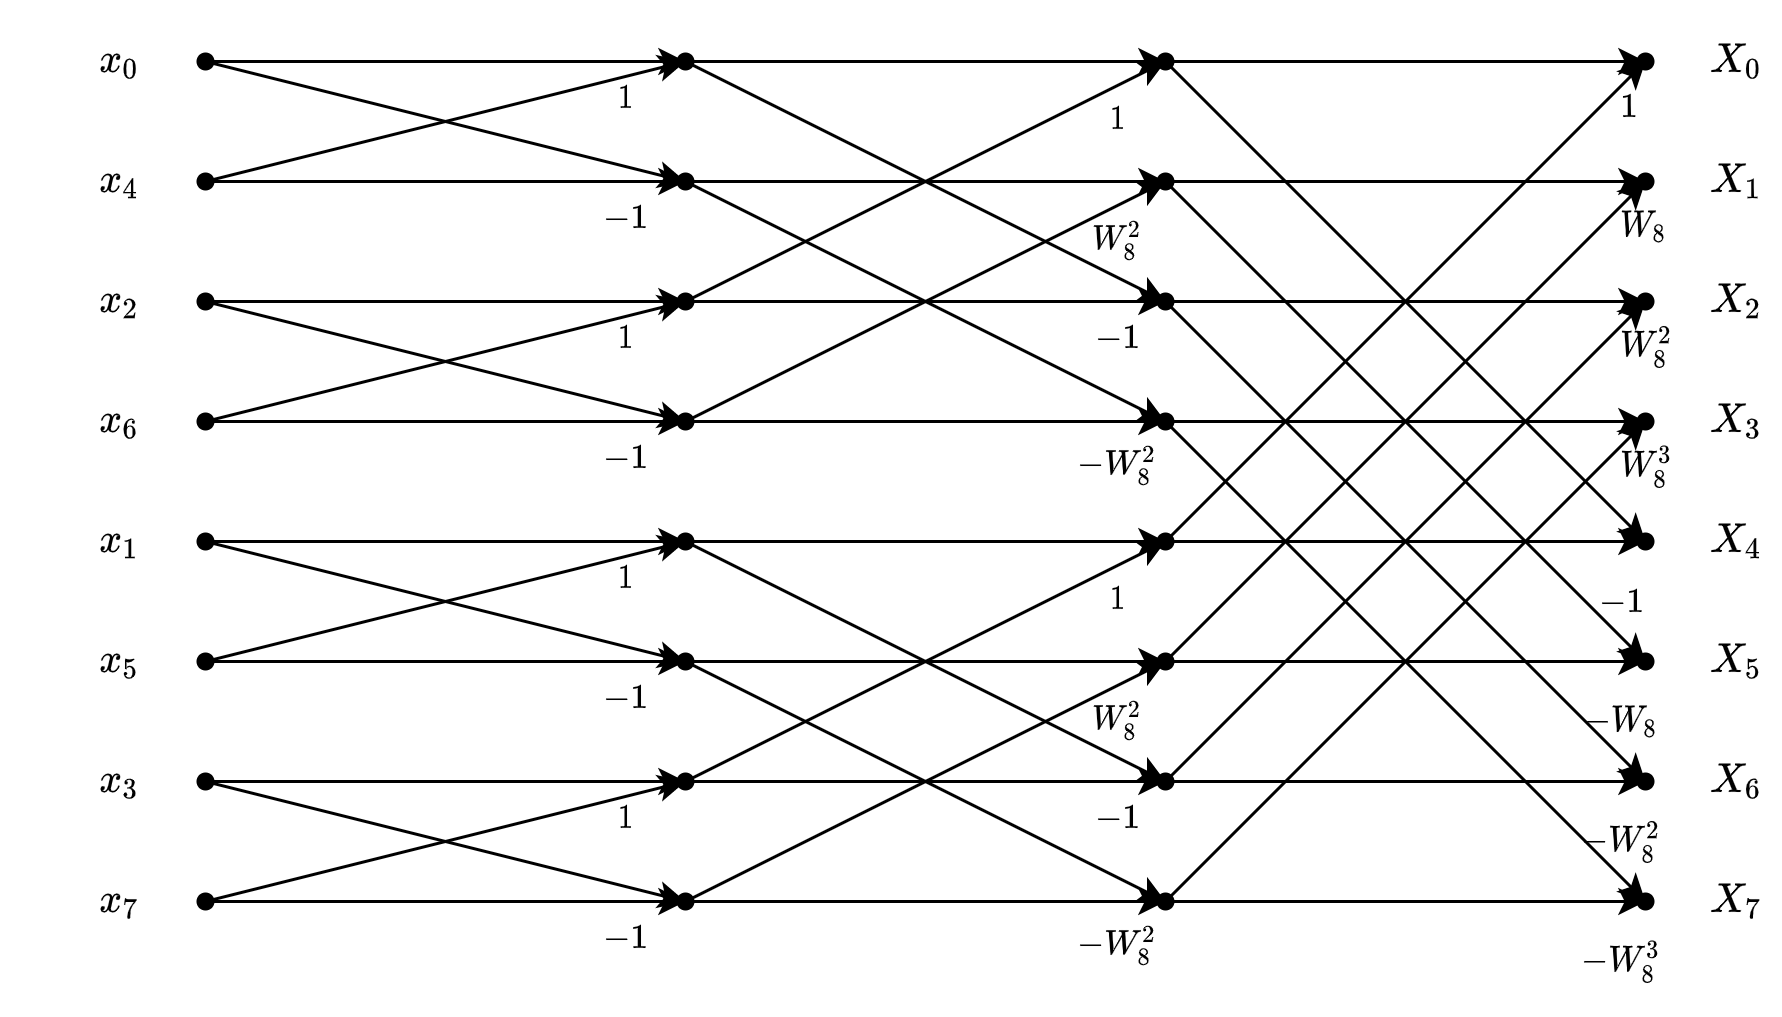
\includegraphics[width=0.8\textwidth]{cooleytukey_8example.png}
	\caption{Computational graph for the Cooley-Tukey (FFT) algorithm for a signal with 8 samples.}
        \label{fig:cooleytukey_8example-png}
    \end{figure}
\end{frame}

\begin{frame}
    \frametitle{The Cooley-Tukey algorithm}
    \begin{algorithm}[H]
	\caption{Recursive-FFT}
	\KwIn{A sequence $\bm{x}$}
	$N \gets |\bm{x}|$ \\
	\If{$N = 1$}{
	    \Return{$\bm{x}$}
	}
	$W_N \gets e^{2 \pi i / N}$ \\
	$W \gets  1$ \\
	$\bm{x}^{(even)} \gets \left( x_0, x_2, \ldots, x_{N-2} \right) $ \\
	$\bm{x}^{(odd)} \gets \left( x_1, x_3, \ldots, x_{N-1} \right) $ \\
	$\bm{X}^{(even)} \gets $ Recursive-FFT$\left( \bm{x}^{(even)}\right) $ \\
	$\bm{X}^{(odd)} \gets $ Recursive-FFT$\left(  \bm{x}^{(odd)}\right) $ \\
	\For{$r\gets 0$ \KwTo $\frac{N}{2} -1$}{
	    $\bm{X}_r \gets \bm{X}^{(even)}_r + W \bm{X}^{(odd)}_r$ \\
	    $\bm{X}_{r + N / 2} \gets \bm{X}^{(even)}_r - W \bm{X}^{(odd)}_r$ \\
	    $W \gets W W_N$
	}
	\Return{$\bm{X}$}
    \end{algorithm}
\end{frame}

\subsection{Complexity of the Cooley-Tukey algorithm}
\begin{frame}
    \frametitle{FFT complexity}
    Define $T\left( n \right) $ the complexity of the Recursive-FFT. Besides the recursion, every call executes $n$ operations. So we can understand its complexity as
    \begin{align*}
	T(n) = & 2T\left( n / 2 \right) + \Theta\left( n \right)  \\
	= & 4T\left( n / 4 \right) + \Theta\left( n \right)  \\
	& \,\vdots \\
	= & \Theta\left( n \log n \right)
    .\end{align*}
    Another way to see this is through the computational graph. Every column requires $n$ multiplications and $n$ summations, besides extra $\frac{n}{2}$ multiplications to compute $W_n^r$. For $n$ a power of 2, we will have $\log n$ levels. Therefore, FFT runs in $\Theta\left( n \log n \right) $.
\end{frame}

\begin{frame}
    \frametitle{FFT complexity}
    Comparing to DFT, it is a huge advance.
    \begin{table}[]
    \begin{tabular}{c|c|c}
    \textbf{N}    & \textbf{DFT} $\Theta(n^2)$ & \textbf{FFT} $\Theta(n \log n)$ \\ \hline
    $8$    & $64$                             & $24$                                  \\ \hline
    $256$  & $65536$                          & $2048$                                \\ \hline
    $4096$ & $\approx 10^7$                 & $\approx 10^4$                      \\
    \end{tabular}
    \end{table}
\end{frame}

\subsection{Efficient Implementation}
\begin{frame}
    \frametitle{Efficient implementation}
    \begin{itemize}
        \item It is usually more efficient to have an iterative implementation rather than a recursive one.
	\item The idea then is to traverse the computational graph from left-to-right, one column at a time.
    \end{itemize}
    \begin{figure}
        \centering
        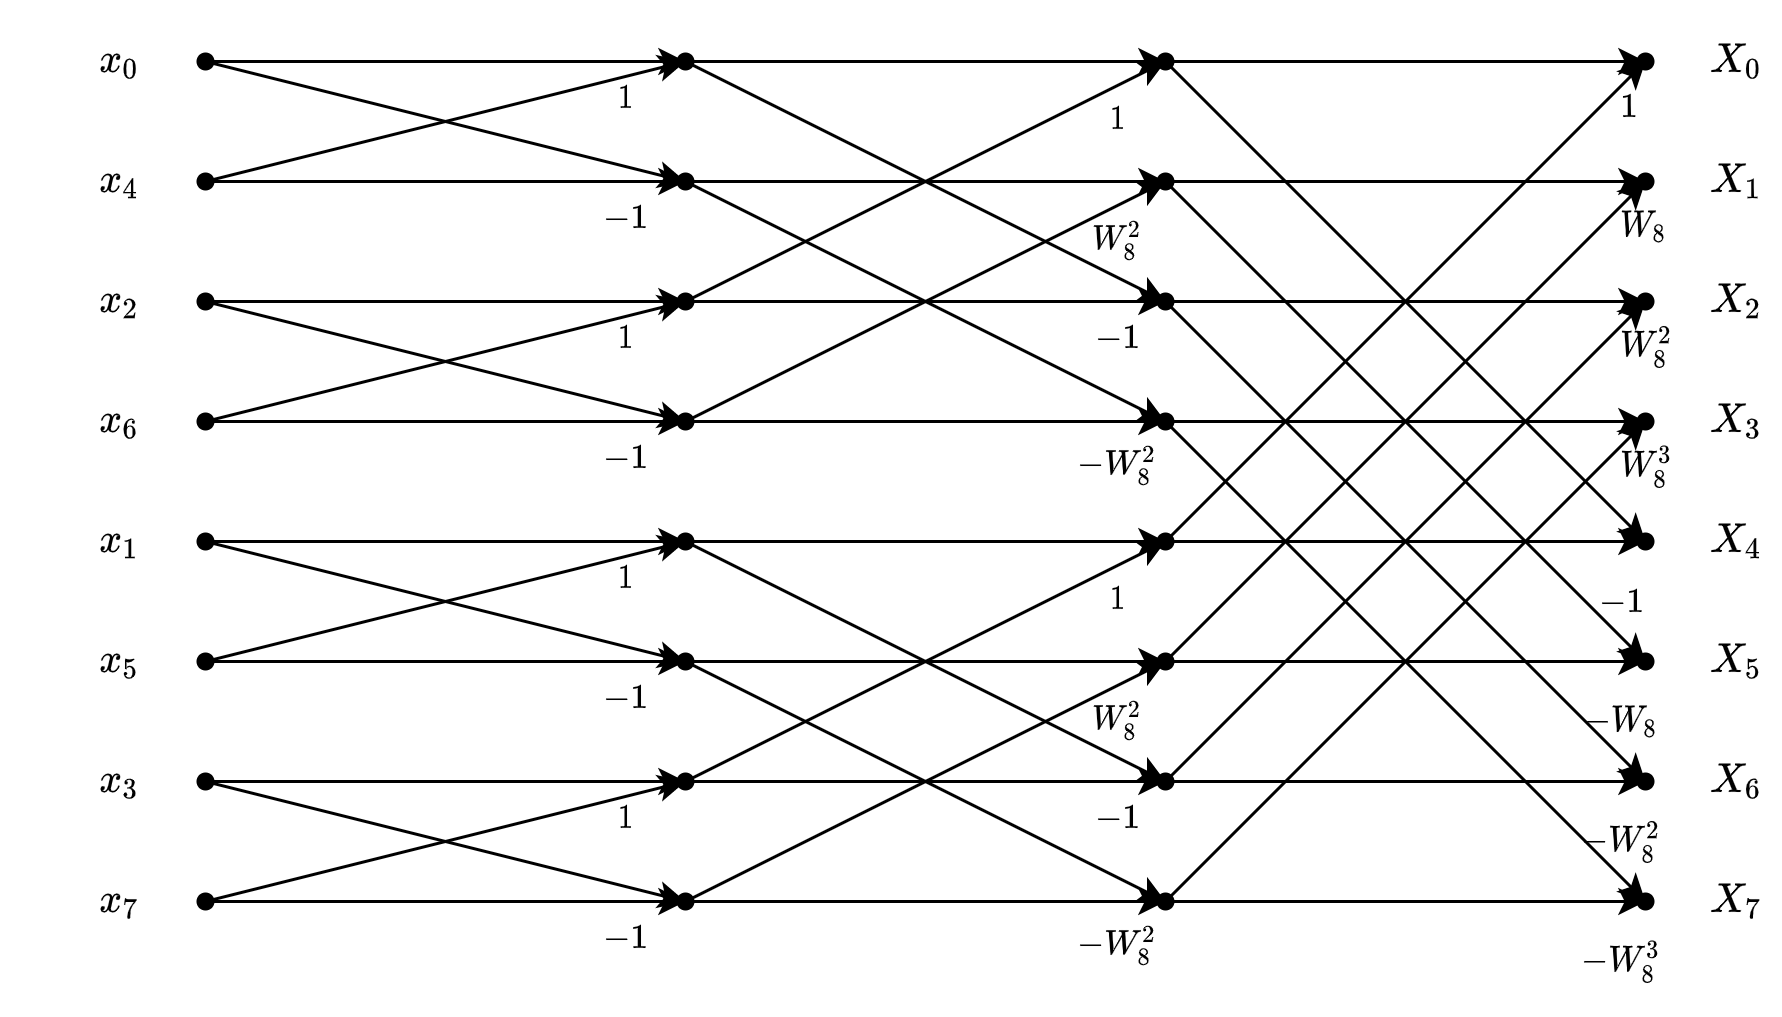
\includegraphics[width=0.6\textwidth]{cooleytukey_8example.png}
    \end{figure}
\end{frame}

\begin{frame}
    \frametitle{Efficient implementation}
    \begin{algorithm}[H]
	\caption{Iterative-FFT}
	\KwIn{A sequence $\bm{x}$}
	$N \gets |\bm{x}|$ \\
	$\bm{X} \gets $ Bit-Reverse-Copy$\left( \bm{x} \right) $ \\

	\For{$s \gets 1$ \KwTo $\log N$}{
	    $M \gets 2^{s}$ // $M$ is the size of the gap of the butterfly \\
	    $W_M \gets e^{\frac{2\pi i}{M}}$ \\

	    \For{$k\gets 0$ \KwTo $N-1$ \KwBy $M$}{
		$W \gets 1$ \\
		\For{$r\gets 0$ \KwTo $\frac{M}{2} -1$}{
		    $u \gets \bm{X}_{k+r}$ \\
		    $t\gets W \bm{X}_{k+r+ M / 2}$ \\
		    $\bm{X}_{k+r} \gets u+t$ \\
		    $\bm{X}_{k+r + M / 2} \gets u-t$ \\
		    $W \gets W W_M$
		}
	    }
	}
	\Return{$\bm{X}$}
    \end{algorithm}
\end{frame}

\begin{frame}
    \frametitle{Efficient implementation}
    \begin{itemize}
	\item The $s$ variable is the column of the computational graph.
	\item 
        \item The Bit-Reverse-Copy reorders the sequence by reversing the index value binary, e.g., $100\to 001$. So it runs $N$ iterations over the array and $n \log n$ iterations to reverse the binary value, which results in $\Theta\left( n \log n \right) $.
	\item 
	\item The indexing is confusing, but a bench test is enough to grasp the ordering of the algorithm.
    \end{itemize}
\end{frame}

\begin{frame}
    \frametitle{Efficient implementation}
    Also, the middle loop can be performed in parallel, as visible in the figure below, which is a great feature for modern computers.
    \begin{figure}
        \centering
        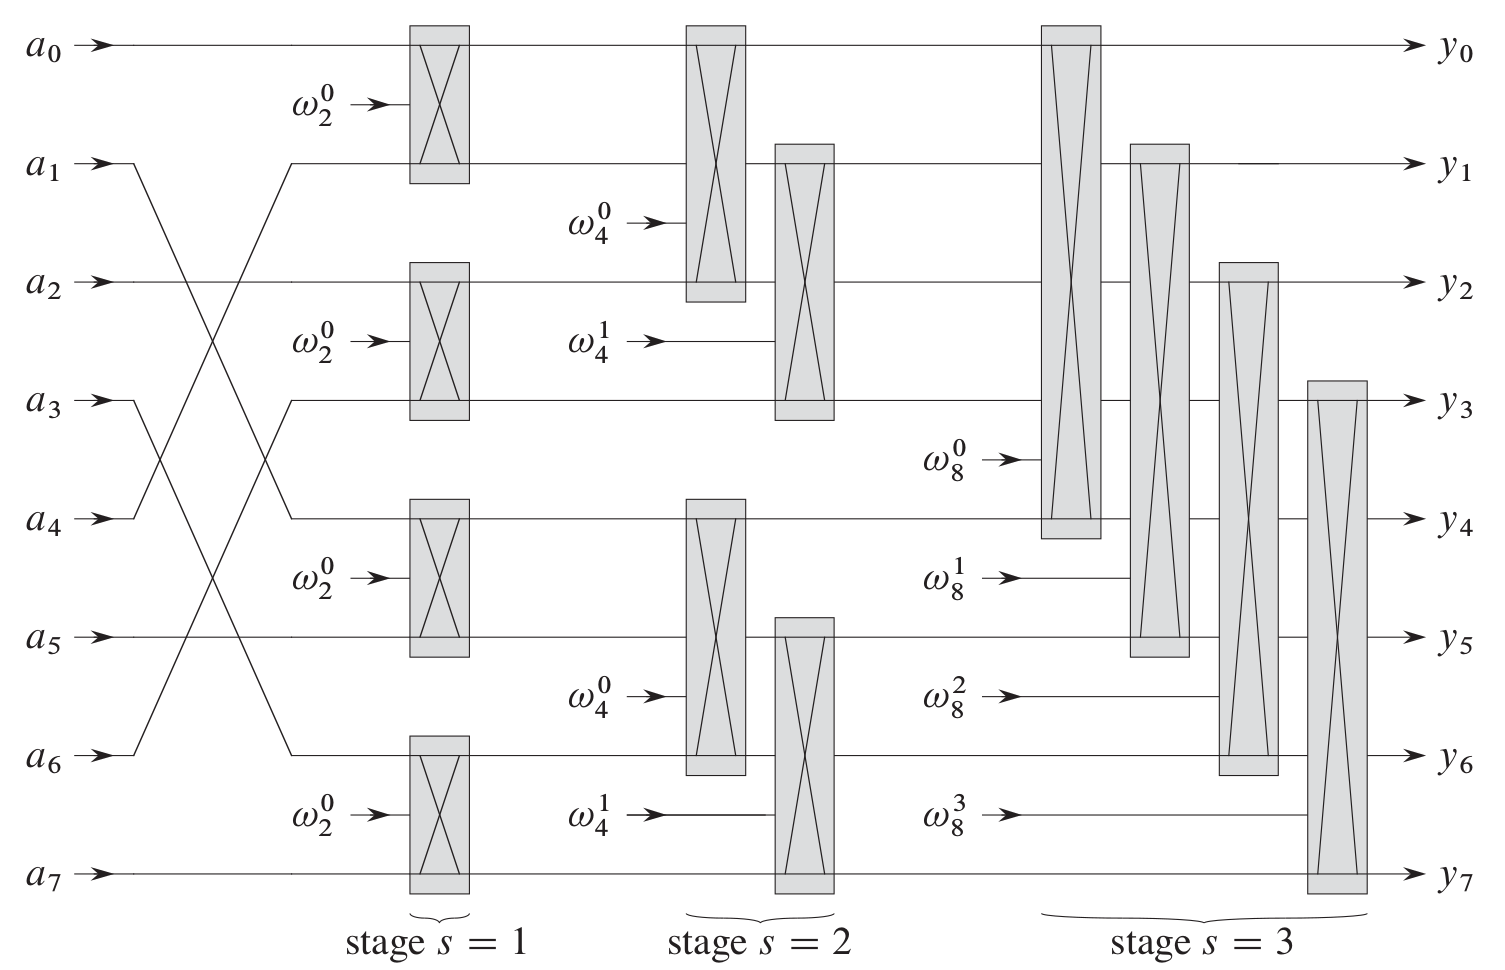
\includegraphics[width=0.8\textwidth]{cormen_fft_parallel.png}
        \caption{Illustration of the Iterative-FFT, by Cormen et al, 2009. $a = \bm{x}$ and $y = \bm{X}$.}
        \label{fig:cormen_fft_parallel-png}
    \end{figure}
\end{frame}

\section{Applications}

\subsection{Convolutions}

\begin{frame}
    \frametitle{Convolutions}
    Given two discrete signals $x_{n}, g_n$, sampled at the same rate, both with size $N$, the circular convolution of both is defined as \[
    x_{n}\circledast g_n = \sum_{k=0}^{N-1} g_k x_{n-k} = c_n
    .\] This operation is, clearly, $\Theta\left( n^2 \right) $.
\end{frame}

\begin{frame}
    \frametitle{Convolutions}
    Luckily, the convolution theorem also applies to the DFT and for circular convolutions, that is, given $x_{n},\,g_n$ and $X_r,\,G_r$, \[
    x_{n} \circledast g_n \xleftrightarrow{\mathcal{F}} X_r G_r
    .\] Thus, we can use the FFT to compute convolutions faster.
\end{frame}

\begin{frame}
    \frametitle{Convolutions}
    As the FFT takes $\Theta\left( n \log n \right) $ and the convolution can be performed as a point-wise multiplication in the frequency domain, i.e., in $\Theta\left( n \right) $, this operation is faster than performing the convolution straight away.
    \begin{figure}
        \centering
        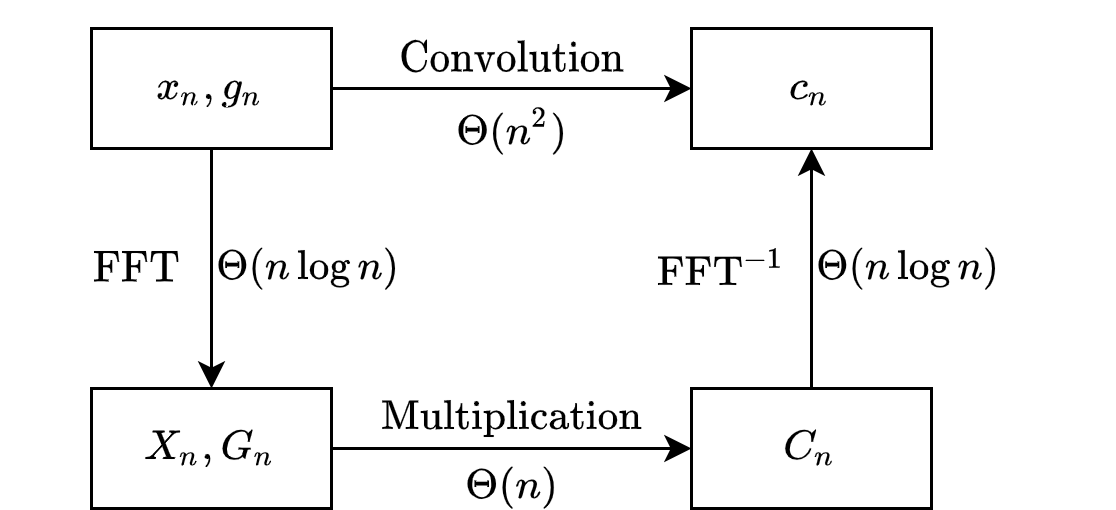
\includegraphics[width=0.8\textwidth]{convolution_fft.png}
        \caption{Convolution steps through the FFT.}
        \label{fig:convolution_fft-png}
    \end{figure}
\end{frame}

\subsection{Multiplication of Polynomials}

\begin{frame}
    \frametitle{Multiplication of polynomials}
    Given two polynomials $A(x),B(x)$ of degrees $N_a,N_b$ resp., we can write them as \[
    A\left( x \right) = \sum_{j=0}^{N_a} a_j x^{j},\, B\left( x \right) = \sum_{j=0}^{N_a} b_j x^{j}
    .\] Their \emph{multiplication} results in a polynomial $C\left( x \right) = A(x)B(x)$, in which usually we compute \[
    C(x) = \sum_{j=0}^{N_a+N_b} c_j x^{j} \implies c_j = \sum_{k=0}^{j} a_k b_{j-k}
.\]
\end{frame}

\begin{frame}
    \frametitle{Multiplication of polynomials}
    \[
    C(x) = \sum_{j=0}^{N_a+N_b} c_j x^{j} \implies c_j = \sum_{k=0}^{j} a_k b_{j-k}
.\] To compute the coefficients of $C(x)$ we will need to multiply every coefficient of $A(x)$ and $B(x)$, it will require $N_aN_b$ multiplications besides the summations, that are \[
1 + 2 + \ldots + \left( N_a+N_b \right) = \frac{\left( N_a+N_b \right) \left( N_a+N_b +1\right) }{2}
.\] 
Therefore, we can say it belongs to $\Theta(n^2)$.
\end{frame}

\begin{frame}
    \frametitle{Point-value representation of polynomials}
    Given a set $\{\left( x_0,y_0 \right) ,\ldots,\left( x_N,y_N \right) \} $ of \emph{distinct} pairs, it is true that there is only one polynomial $A(x)$ of degree $N$ such that \[
	y_k = A(x_k),\, k = 0,\ldots ,N
    .\] Thus, this is a valid representation of a polynomial.
\end{frame}

\begin{frame}
    \frametitle{Point-value representation of polynomials}
    \begin{itemize}
        \item It is clear that in this representation, one can compute the multiplication of the polynomials in $\Theta\left( n \right) $.
	\item
	\item Still, this representation is not very useful, as it does not provide an easy way to evaluate the polynomial at values from its domain.
	\item
	\item Therefore, the question arises: \emph{How expensive it is to go to and from the point-value representation?}
    \end{itemize}
\end{frame}

\begin{frame}
    \frametitle{Point-value representation of polynomials}
    To the point-value representation, one can evaluate random distinct $N$ points. As each evaluation takes $N$ operation, this will be a $\Theta\left( n^2 \right) $.
    \linebreak \linebreak
    From the point-value representation, one can use \emph{Lagrange's formula}: \[
	A(x) = \sum_{k=0}^{N} y_k \frac{\prod_{j\neq k} \left( x-x_j \right)  }{\prod_{j\neq k} \left( x_k-x_j \right)}
    ,\] which is $\Theta\left( n^2 \right) $.
    So this ends but being at least as expensive as computing the coefficients of the resulting polynomial.
\end{frame}

\begin{frame}
    \frametitle{Point-value representation of polynomials}
    Now, suppose we want to evaluate the polynomial at $\{W_{N+1}^{0},\ldots,W_{N+1}^{N}\} $ (remember that $W_{N+1} = e^{-\frac{2\pi i}{N+1}}$). Then, we want to compute \[
    y_k = A\left( W_{N+1}^{k} \right) = \sum_{j=0}^{N} a_j W_{N+1}^{kj}
    ,\] which means that $\left( y_0,\ldots,y_N \right)$ is \emph{precisely} the DFT of $\left( a_0,\ldots,a_N \right) $.
\end{frame}

\begin{frame}
    \frametitle{Point-value representation of polynomials}
    As multiplying polynomials with the point-value representation does not change their evaluation points, one can also use the inverse DFT to get back to the coefficient representation.
    \linebreak \linebreak
    Thus, thanks to the FFT, we can go back-and-forth between the two representations in $\Theta\left( n \log n \right) $.
\end{frame}

\begin{frame}
    \frametitle{Point-value representation of polynomials}
    \begin{figure}
        \centering
        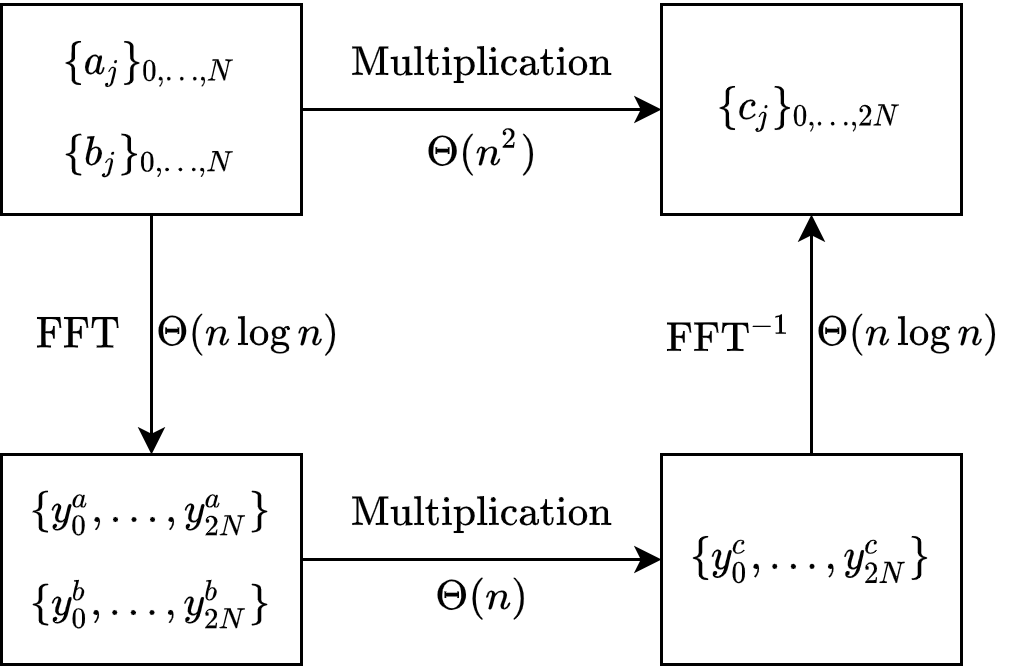
\includegraphics[width=0.8\textwidth]{poly_mult.png}
        \caption{Steps to multiply two polynomials using the FFT.}
        \label{fig:poly_mult-png}
    \end{figure}
\end{frame}

\section{Conclusion}
\begin{frame}
    \frametitle{Takeaways}

    \begin{itemize}
        \item The DFT is broadly used in many different areas, with much broader applicability than signal analysis
	\item
	\item Being able to compute it in $\Theta\left( n \log n \right) $ allows for the computation of many solutions in reasonable time.
	\item
	\item As we saw it in the examples, the FFT is a nice tool to have in hand as it can be applied to very basic and common operations
    \end{itemize}
\end{frame}

\begin{frame}
    \begin{center}
	Thank you!
    \end{center}
\end{frame}

\end{document}
